{%\color{red}
\chapter{Performance models}

\section{Roofline model}

The Roofline model is an intuitive visual model that shows for given processor the upper bound of performance. The model is based on an idea that a compute kernel performs some computations with data that are read and written from/to memory. Performance of the kernel is bound by the ability of the CPU to perform computations (peak performance) and the ability to read and write data (memory bandwidth).
The model is typically shown for a given processor as a graph with arithmetic intensity on the x-axis and performance on the y-axis. The arithmetic intensity $I [F/B]$ (code balance $B_c = I^{-1}$) is a ratio between numerical operations and memory traffic. Typically we are interested in floating point operations, so it is shown in FLOPs/B.
The performance upper bound $P [F/s]$ is either the peak performance $P_{peak} [F/s]$ of the processor, it simply cannot perform more computations, or it could compute more, but has to wait for data being transferred from or to memory, then the limit is the memory bandwidth $b_s [B/s]$.
These can be written as

\begin{equation}
   P = min(P_{peak}, I \cdot b_s) = min(P_{peak}, b_s / B_c).
\end{equation}

The model can be improved by adding ceilings. The peak performance can be achieved only when using all cores, the code is vectorized and fused multiply-add (FMA) instructions are used. If for example vectorization is not possible, only $\frac{P_{peak}}{4}$ can be achieved. And if FMA is not used, it further limits the performance to a half.
And similar with memory bandwidth. Modern processors are not able to use the whole memory bandwidth with a single core. \todol{todo} 

In the figure \ref{fig:roofline_emmy} a roofline model of an Intel Ivy Bridge processor is shown with with different memory bandwidth for 1 and 10 cores and different max performance with and without vectorization (AVX) and FMA. \todol{todo}

\begin{figure}[H]
   \centering
   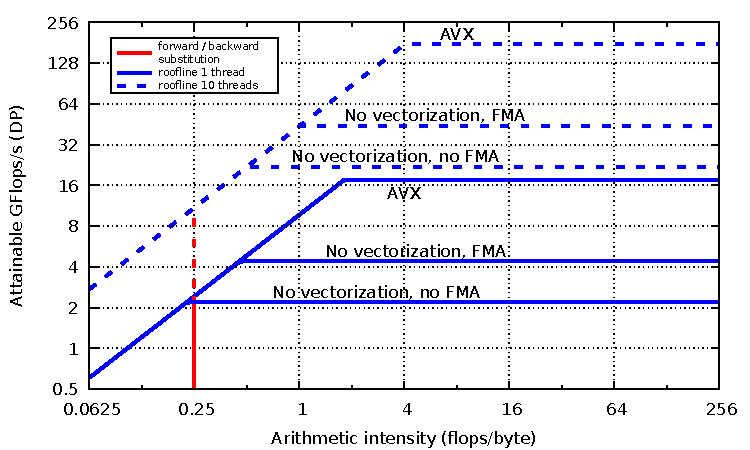
\includegraphics[width=0.7\textwidth,clip=true]{images/roofline_emmy_Xeon2660v2}
   \caption{Roofline model of the  Intel Xeon E5-2660 v2 CPU.}
  \label{fig:roofline_emmy}
\end{figure}

%This upper bound may not be feasible by given kernel. In order to make the model more precise, different ceilings limiting the performance or memory bandwidth can be introduced.
%For example if only single core is used, the full memory bandwidth can not be achieved, so it is reasonable to adjust it accordingly. Also the maximum performance depends on the code and instruction set used by compiler. To be able to achieve the peak performance on modern CPU, all cores must be used, the generated code must be vectorized and fused multiply add (FMA) instructions must be used. 

\section{Extended roofline model}
\label{sec:mrm}

The roofline model is very useful for code that is either completely sequential or completely parallel. However when the number of threads changes during execution, the roofline model cannot be used, because the attainable performance $P_{max}$ and memory bandwidth $b_s$ depend on number of threads used.

We modified the roofline model such that it models independently the work done sequentially and in parallel.
The formula used for combination of $1$ and $t$ threads is
%
\begin{equation}
  p^{a}(t) 
  = \frac{
      f
    }{
     \frac{d_a^p(t) }{  b(t) } + \frac{ d_a^s(t) }{ b(1) }
    } \left[ \frac{\text{flop}}{s} \right],
\end{equation}
%
where $f$ denotes the total number of floating point operations,
$b(t)$ is the attainable memory bandwidth with $t$ threads,
$b(1)$ is the attainable memory bandwidth with $1$ thread,
$d_a^p(t)$ the data volume of nonzeros and indices made up by the parallel 
parts, and $d_a^s(t)$ the data volume made up by the nonzeros and indices of the
sequential computation (separator). \todol{todo}

\section{ECM model}


}